% \documentclass{article}
% \usepackage[utf8]{inputenc}

% \title{AProf Hw1}
% \author{André Lopes Rodrigues}
% \author{Duarte Calado Almeida}
% \date{December 2022}

% \begin{document}

% \maketitle

% \section{Introduction}

% \end{document}

\documentclass{exam}

\usepackage{titling}
\usepackage{amsmath}
\usepackage{amsfonts}
\usepackage{mathtools}
\usepackage{float}
\usepackage{tikz}
\usepackage{graphicx}
\usepackage{subfig}
\usepackage{inconsolata}
\usepackage{tikz}
\usepackage{physics}
\usepackage{amsthm}
\usepackage[font={small}]{caption}
\usepackage{courier}
\usepackage{amsbsy}
\usepackage{comment}

\DeclareMathOperator*{\argmax}{argmax}

\graphicspath{ {./pictures} }

\setlength{\droptitle}{-5em}   

%\renewcommand{\questionlabel}{\textbf{~\thequestion)}}
%\renewcommand{\subpartlabel}{\thesubpart)}
%\DeclarePairedDelimiterX{\norm}[1]{\lVert}{\rVert}{#1}

\newcommand*{\horzbar}{\rule[.5ex]{2.5ex}{0.5pt}}

\newenvironment{shiftedflalign*}{%
    \start@align\tw@\st@rredtrue\m@ne
    \hskip\parindent
}{%
    \endalign
}

\newcommand{\brows}[1]{%
  \begin{bmatrix}
  \begin{array}{@{\protect\rotvert\;}c@{\;\protect\rotvert}}
  #1
  \end{array}
  \end{bmatrix}
}

\newcommand{\rotvert}{\rotatebox[origin=c]{90}{$\vert$}}
\newcommand{\rowsvdots}{\multicolumn{1}{@{}c@{}}{\vdots}}

\newtheorem{lemma}{Lemma}

\title{%
  Homework 2\\
  \vspace{0.5em}
  \large Deep Learning \\
  \vspace{0.5em}
  \normalsize Group 5} \\
\author{
  Duarte Calado de Almeida\\
  95565
  \and
  André Lopes Rodrigues\\
  96576
}
\date{}

\cfoot{\thepage}

\begin{document}
    \maketitle
    
    \begin{tikzpicture}[overlay, remember picture]
        \node[xshift=3.5cm,yshift=-2cm] at (current page.north west) {
\includegraphics[scale = 0.35]{logo_ist.jpg}};
    \end{tikzpicture}

    \vspace{-4.2em}

    \noindent\makebox[\linewidth]{\rule{18cm}{0.4pt}}

        The contribution of each member was as follows:
         André Rodrigues did Questions 1.1 (a), 1.1 (c), 2.1, 2.2, 2.4 and 3.1, 
         while Duarte Almeida did Questions 1.1 (b), 1.2, 2.3, 2.5, 3.2 and 3.3. The elaboration of this report was made in colaboration by both students.\\
    \vspace{-0.5cm}
    \noindent\makebox[\linewidth]{\rule[1ex]{18cm}{0.4pt}}
    

  
    \section*{Question 1}
    \begin{questions}
        \question
        \begin{parts}
            \part %1.1(a)
                For a convolutional layer with a single $M \times N$ filter with no padding and a stride of $s$, the element $(i, j)$ of the output $\vb*{z}$ can be written as:
                \[
                z(i, j) = \sum_{m = 1}^{M} \sum_{n = 1}^{N} w(m, n) x(row(i) - 1 + m, col(j) - 1 + n)
                \]
                where $row$ and $col$ are sequences of row and column indices, respectively, such that $row(i) = 1 + s(i - 1)$  and $col(j) = 1 + s(j - 1)$. Given that $1 \le m \le M$, $1 \le n \le N$ and that the maximum row and column indices of $\vb*{x}$ are respectively $H$ and $W$, we have that the maximum row index of $\vb*{z}$ is the largest integer $i$ that satisfies:
                \[
                row(i) - 1 + M \le H \Leftrightarrow  1 + s(i - 1) - 1 + M \le H \Leftrightarrow s(i - 1) \le H - M \Leftrightarrow 
                i \le \frac{H - M}{s} + 1
                \]
                that is, the number of rows in $z$ is $\lfloor\frac{H - M}{s}\rfloor + 1$. Analogously, the maximum column index in $\vb*{z}$ is the largest integer $j$ that satisfies $col(j) - 1 + N \le W$, which is $\lfloor\frac{H - M}{s}\rfloor + 1$. \textbf{Thus, $\vb*{z}$ is a $(H - M + 1) \times (W - N + 1)$ matrix}.
            \part %1.1(b)
                 Without loss of generality, consider the vectorization operation where, for a matrix $\vb*{x} \in \mathbb{R}^{X \times Y}$, $\vb*{x}(i, j) = \vb*{x^\prime}_{X(i - 1) + j}$, i.e., one that is made row-wise. \\
                 To prove that there exists a matrix $\vb*{M} \in \mathbb{R}^{HW \times H^{\prime}W^{\prime}}$ such that $\vb*{z^\prime} = \vb*{Mx^\prime}$, we first note that $\vb*{x}^{\prime} \in \mathbb{R}^{HW}$ and $\vb*{z}^{\prime} \in \mathbb{R}^{H^{\prime}W^{\prime}}$, following the proof above. It then suffices to prove that, for every $i \in \{1, \dots, H^{\prime}W^{\prime}\}$, $z^{\prime}_{i} = \vb*{m}^{T}\vb*{x^{\prime}}$, i.e., $z^{\prime}_{i}$ is a linear combination of the entries of $\vb*{x}^{\prime}$. \\
                 For every $i \in \{1, \dots, H^{\prime}W^{\prime}\}$, define both $\alpha_{i} = \lfloor \frac{i - 1}{H^{\prime}} \rfloor + 1$ and $\beta_{i} = ((i - 1) \mod W^{\prime} + 1)$ that make $z^{\prime}_{i} = z(\alpha_i, \beta_i)$. We then have that:
                 \begin{align*}
                 z^{\prime}_i = z(\alpha_i, \beta_i) &= \sum_{m = 1}^{M} \sum_{n = 1}^{N} w(m, n) x(\alpha_i - 1 + m, \beta_i - 1 + n) \\
                 &= \sum_{m = 1}^{M} \sum_{n = 1}^{N} w(m, n) x^{\prime}_{H(\alpha_i - 2 + m) + (\beta_i - 1 + n)}
                 \end{align*}
                 thus proving the desired result. \\
                 To specify each entry $M(i, j)$ of $\vb*{M}$, note that $\vb*{z}^{\prime} = \vb*{Mx^{\prime}}$ implies that $\nabla_{\vb*{x}^{\prime}}\vb*{z}^{\prime} = \vb*{M}^T$ and, hence, $\frac{\partial z^{\prime}_{i}}{\partial x^{\prime}_{j}} = M^T(j, i) = M(i, j)$. Let $\alpha$, $\beta$, $\gamma$ and $\delta$ be numbers that make $z^{\prime}_i = z(\alpha, \beta)$ and $x^{\prime}_j = x(\gamma, \delta)$ and which are defined in the same fashion as before. We then have that 
                 \begin{align*}
                 M(i, j) = \frac{\partial z^{\prime}_{i}}{\partial x^{\prime}_{j}}  = \frac{\partial z(\alpha, \beta)}{\partial x(\gamma, \delta)} &= \frac{\partial}{\partial x(\gamma, \delta)} \left(\sum_{m = 1}^{M} \sum_{n = 1}^{N} w(m, n) x(\alpha - 1 + m, \beta - 1 + n) \right) \\
                 \end{align*}
                 For $x(\gamma, \delta)$ to appear sum above, there must exist some natural numbers $m^{*}$ and $n^{*}$ that cumulatively satisfy: \\
                 \begin{equation*}
                     \begin{cases}
                        \gamma = \alpha - 1 + m^{*} \wedge 1 \le m^{*} \le M \\
                        \delta = \beta - 1 + n^{*} \wedge 1 \le n^{*} \le N
                     \end{cases} \Rightarrow 
                      \begin{cases}
                        m^{*} = \gamma - \alpha + 1  \wedge 1 \le m^{*} \le M \\
                        n^{*} = \delta - \beta + 1 \wedge 1 \le n^{*} \le N
                     \end{cases}  \Rightarrow
                    \begin{cases}
                        0 \le \gamma - \alpha \le M - 1 \\
                        0 \le \delta - \beta \le N - 1
                     \end{cases}
                \end{equation*}
                Defining 
                \begin{align*}
                    \alpha &= \lfloor \frac{i - 1}{H^{\prime}} \rfloor + 1 \\ 
                    \beta &= ((i - 1) \mod W^{\prime} + 1) \\ 
                    \gamma &= \lfloor \frac{j - 1}{H} \rfloor + 1 \\
                    \delta &= ((j - 1) \mod W + 1)
                \end{align*}
                we can now formalize a definition for $M(i, j)$:
                
                \begin{align*}
                    M(i, j) = 
                    \begin{cases}
                        w(\gamma - \alpha + 1, \delta - \beta + 1), & 0 \le \gamma - \alpha \le M - 1 \: \wedge \: 0 \le \delta - \beta \le N - 1 \\
                        0, & \text{otherwise}
                    \end{cases}
                \end{align*}
              
            \part %1.1(c)
                All the operations with trainable parameters that take place in this network are a convolution with a $M \times N$ filter and the linear map present in the fully connected layer at the end. The last operation takes as input the vectorization of the result of the $2 \times 2$ max-pooling operation with stride 2, which has size
                \[ H^{\prime\prime} \times W^{\prime\prime} 
                = \left(\left\lfloor \frac{H^{\prime} - 2}{2} \right\rfloor + 1\right) \times \left(\left\lfloor \frac{W^{\prime} - 2}{2} \right\rfloor + 1\right) 
                = \left\lfloor \frac{H^{\prime}}{2} \right\rfloor \times \left\lfloor \frac{W^{\prime}}{2} \right\rfloor 
                = \left\lfloor \frac{H - M + 1}{2} \right\rfloor \times \left\lfloor \frac{W - N + 1}{2} \right\rfloor
                \]
                and maps it to $\mathbb{R}^3$. Hence, this architectures yields a total number of parameters of $MN + 3 \left(\lfloor \frac{H - M + 1}{2} \rfloor \times \lfloor \frac{W - N + 1}{2} \rfloor \right)$ (ignoring bias terms). \\
                If instead of the convolutional and max-pooling layers we had a single fully connected layer yielding an output with the same dimension as $\vb*{h}_2$ (i.e., mapping $\mathbb{R}^{HW}$ to $\mathbb{R}^{H^{\prime\prime}W^{\prime\prime}}$), we would have 
                \[
                HW \times H^{\prime\prime}W^{\prime\prime} + 3H^{\prime\prime}W^{\prime\prime} = (HW + 3) \left(\left\lfloor \frac{H - M + 1}{2} \right\rfloor \times \left\lfloor \frac{W - N + 1}{2} \right\rfloor\right)
                \]
                parameters (ignoring bias terms). Notice that the space complexity of the first solution in terms of the image size is $O(HW)$, which is clearly superior to the complexity of $O(H^2 W^2)$ that the solution that uses only fully connected layers exhibits.
                
        \end{parts}
        %\newpage
        \question %1.1(c)
        Considering that all projection matrices are equal to 1, the matrices of queries, keys and values are defined as:
        \begin{align*}
            \vb*{Q} &= \vb*{x^{\prime}} \; \vb*{W_Q}  = \vb*{x^{\prime}} \cdot 1 = \vb*{x^{\prime}} \\
            \vb*{K} &= \vb*{x^{\prime}} \; \vb*{W_K} = \vb*{x^{\prime}} \cdot 1 = \vb*{x^{\prime}}\\
            \vb*{V} &= \vb*{x^{\prime}} \; \vb*{W_V} = \vb*{x^{\prime}} \cdot 1 = \vb*{x^{\prime}} 
        \end{align*}
        and, as such, given that the length of query/key vectors satisfies $d_{\vb*{K}} = 1$, the matrix of attention probabilities is defined as:
        \[
        \vb*{P} = \text{softmax}\left(\frac{\vb*{Q}\vb*{K}^T}{\sqrt{d_{\vb*{K}}}}\right) = \text{softmax}(\vb*{x^{\prime}}\vb*{x^{\prime}}^T)
        \]
        which means that each element of $\vb*{P}$ is defined as:
        \[
        P_{ij} = \frac{\exp{x^{\prime}_i x^{\prime}_j}}{\sum_{k = 1}^{HW}\exp{x^{\prime}_i x^{\prime}_k}}
        \]
        Thus, $\vb*{P}$ can be seen as an entry-wise division of two matrices, $\mathcal{M}$, and $\mathcal{N}$, where
        \[
        \mathcal{M}_{ij} = \exp{x^{\prime}_i x^{\prime}_j} \Rightarrow \mathcal{M} = \exp{\vb*{x^{\prime}}\vb*{x^{\prime}}^T}
        \]
        where the exponential is taken entry-wise. Moreover:
        \[
        \mathcal{N}_{ij} =\sum_{k = 1}^{HW}\exp{x^{\prime}_i x^{\prime}_k }\Rightarrow \mathcal{N} = 
        \begin{bmatrix}
            \sum_{k = 1}^{HW}\exp{x^{\prime}_1 x^{\prime}_k} \\
            \sum_{k = 1}^{HW}\exp{x^{\prime}_2 x^{\prime}_k} \\
            \vdots \\
            \sum_{k = 1}^{HW}\exp{x^{\prime}_{HW} x^{\prime}_k}
        \end{bmatrix}
        \begin{bmatrix}
            1, 1, \dots 1
        \end{bmatrix} = 
        \exp{\vb*{x^{\prime}}\vb*{x^{\prime}}^T} \mathbf{1} \mathbf{1}^T
        \]
        Hence, $\vb*{P}$ can be written in matrix form as
        \[
        \vb*{P} = \frac{\exp{\vb*{x^{\prime}}\vb*{x^{\prime}}^T}}{ \exp{\vb*{x^{\prime}}\vb*{x^{\prime}}^T} \mathbf{1} \mathbf{1}^T}
        \]
        where division and exponentiation are performed in an entry-wise fashion.
        Given that the attention output $\vb*{Z}$ is defined as $\vb*{PV}$, it can be expressed in terms of $\vb*{x^{\prime}}$ in the following manner:
        \[
        \vb*{Z} = \vb*{PV} = \frac{\exp{\vb*{x^{\prime}}\vb*{x^{\prime}}^T}}{ \exp{\vb*{x^{\prime}}\vb*{x^{\prime}}^T} \mathbf{1} \mathbf{1}^T} \; \vb*{x^{\prime}}
        \]
        having the $i$-th in the following form ($i \in \{1, \dots, HW\})$:
        \[
         Z_{i} = \frac{\sum_{j = 1}^{HW}\exp{x^{\prime}_i x^{\prime}_j} x^{\prime}_j}{\sum_{k = 1}^{HW}\exp{x^{\prime}_i x^{\prime}_k}}
        \]
                  
    \end{questions}

    \section*{Question 2}

    \begin{questions}
        \question %2.1
            A Convolutional Neural Network (CNN) has fewer parameters than a fully connected network with the same input size and same number of classes because of the way that the layers that make up the network perform computations.
            In a fully connected network, every neuron of a layer is connected to every neuron of the layer before, with the number of parameters of the layer being obtained by multiplying the number of units in the previous layer by the number of units in the current layer. This means that by stacking additional layers, the number of parameters will grow in a rapid manner.
            In contrast, a CNN computes a convolution between a kernel and a shifting image window instead of taking into account the input in its integrity, with the size of the kernel being usually much smaller than that of the image. Even though CNNs also contain fully connected layers, they usually appear in later stages of the network pipeline, and as such their number of units is much smaller than the size of the input that is fed to the network.
            
        \question %2.2
            On one hand, the use of filters in CNNs configures an operation that takes into account spatial structure, and as such is successful in capturing features that are relevant to the discrimination of the contents of an image (e.g., characteristic edges in characters and numbers). On another hand, the use of pooling layers endows CNNs with the capability of recognizing objects regardless of their shift, rotation and scale variability. \\
            Fully connected layers are insensitive to spatial structure in virtue of the blind vectorization of the input and the use of successive afine maps and activation functions that consider all of the inputs at all stages of the classification pipeline. Thus, they are usually outperformed by CNNs in image classification tasks, such as recognition of numbers and characters, among others.
        \question %2.3 
            In the absence of spatial correlation and structure, the architecture of CNNs may be underparametrized in comparison with neural networks of fully connected layers and as such may not be able to achieve a level of generalization in such tasks as the latter does. The explanation for that lies in the possibility that various spatially uncorrelated inputs may be now jointly relevant to the extraction of an important feature that would go unrecognized in CNNs due to the inexistence of an output unit that would weigh said units in some convolutional layer.

        \question
            The convolutional network was implemented and tested for 20 epochs, using Adam tuning with the following learning rate values.
            
            \begin{table}[h!]
                \centering
                \begin{tabular}{c|ccccc}
                    &                                     & Learning Rate                      &                 &  &  \\ \cline{2-4}
                    & \multicolumn{1}{c|}{0.00001}          & \multicolumn{1}{c|}{0.0005}          & 0.01             &  &  \\ \cline{1-4}
                    Validation Accuracy & \multicolumn{1}{c|}{0.9559} & \multicolumn{1}{c|}{0.9843} & 0.9298 &  & 
                \end{tabular}
            \end{table}
        
            The best observed configuration was the one with a learning rate of 0.0005.
            The plots of the training loss and validation accuracy over the number of epochs for that configuration are shown below.
    
            \begin{figure}[H]
                \centering
                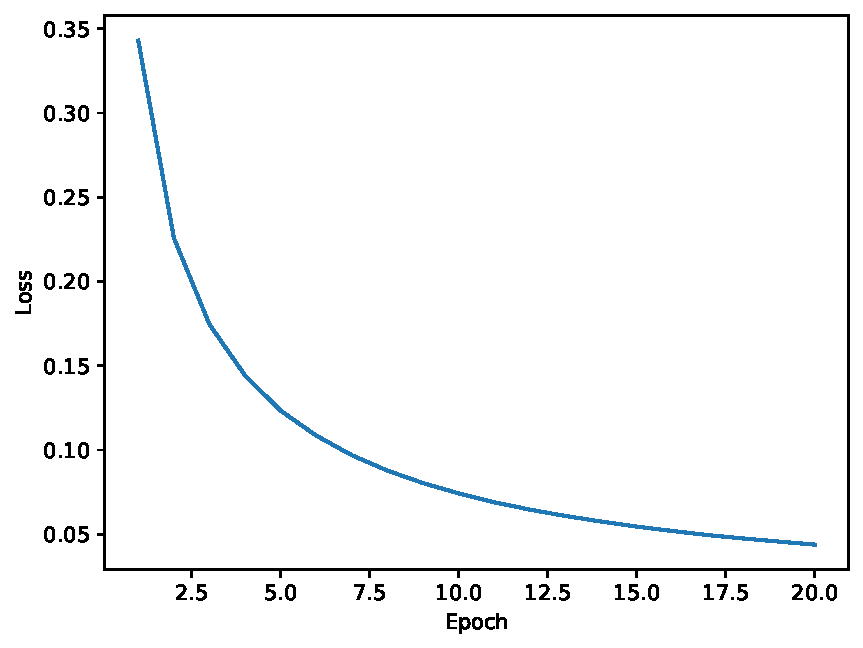
\includegraphics[scale=0.6]{CNN-training-loss-0.0005-0.3-0-adam.pdf}
                \caption{Training Loss over 20 epochs for $\eta = 0.0005$}
                \label{}
            \end{figure}
    
            \begin{figure}[H]
                \centering
                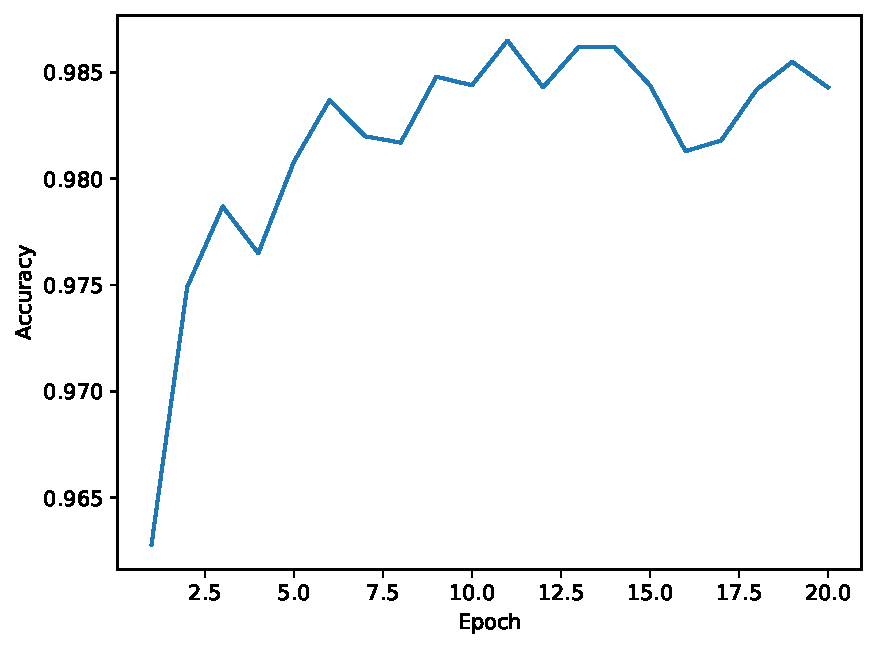
\includegraphics[scale=0.6]{CNN-validation-accuracy-0.0005-0.3-0-adam.pdf}
                \caption{Validation Accuracy over 20 epochs for $\eta = 0.0005$}
                \label{}
            \end{figure}
        \clearpage
        \question
            The obtained activations maps and the corresponding original example are as follows:

            % \begin{figure}[h]
            % \centering
            %     \begin{minipage}[c]{0.5\linewidth}
            %     \hspace*{-2cm}   
            %     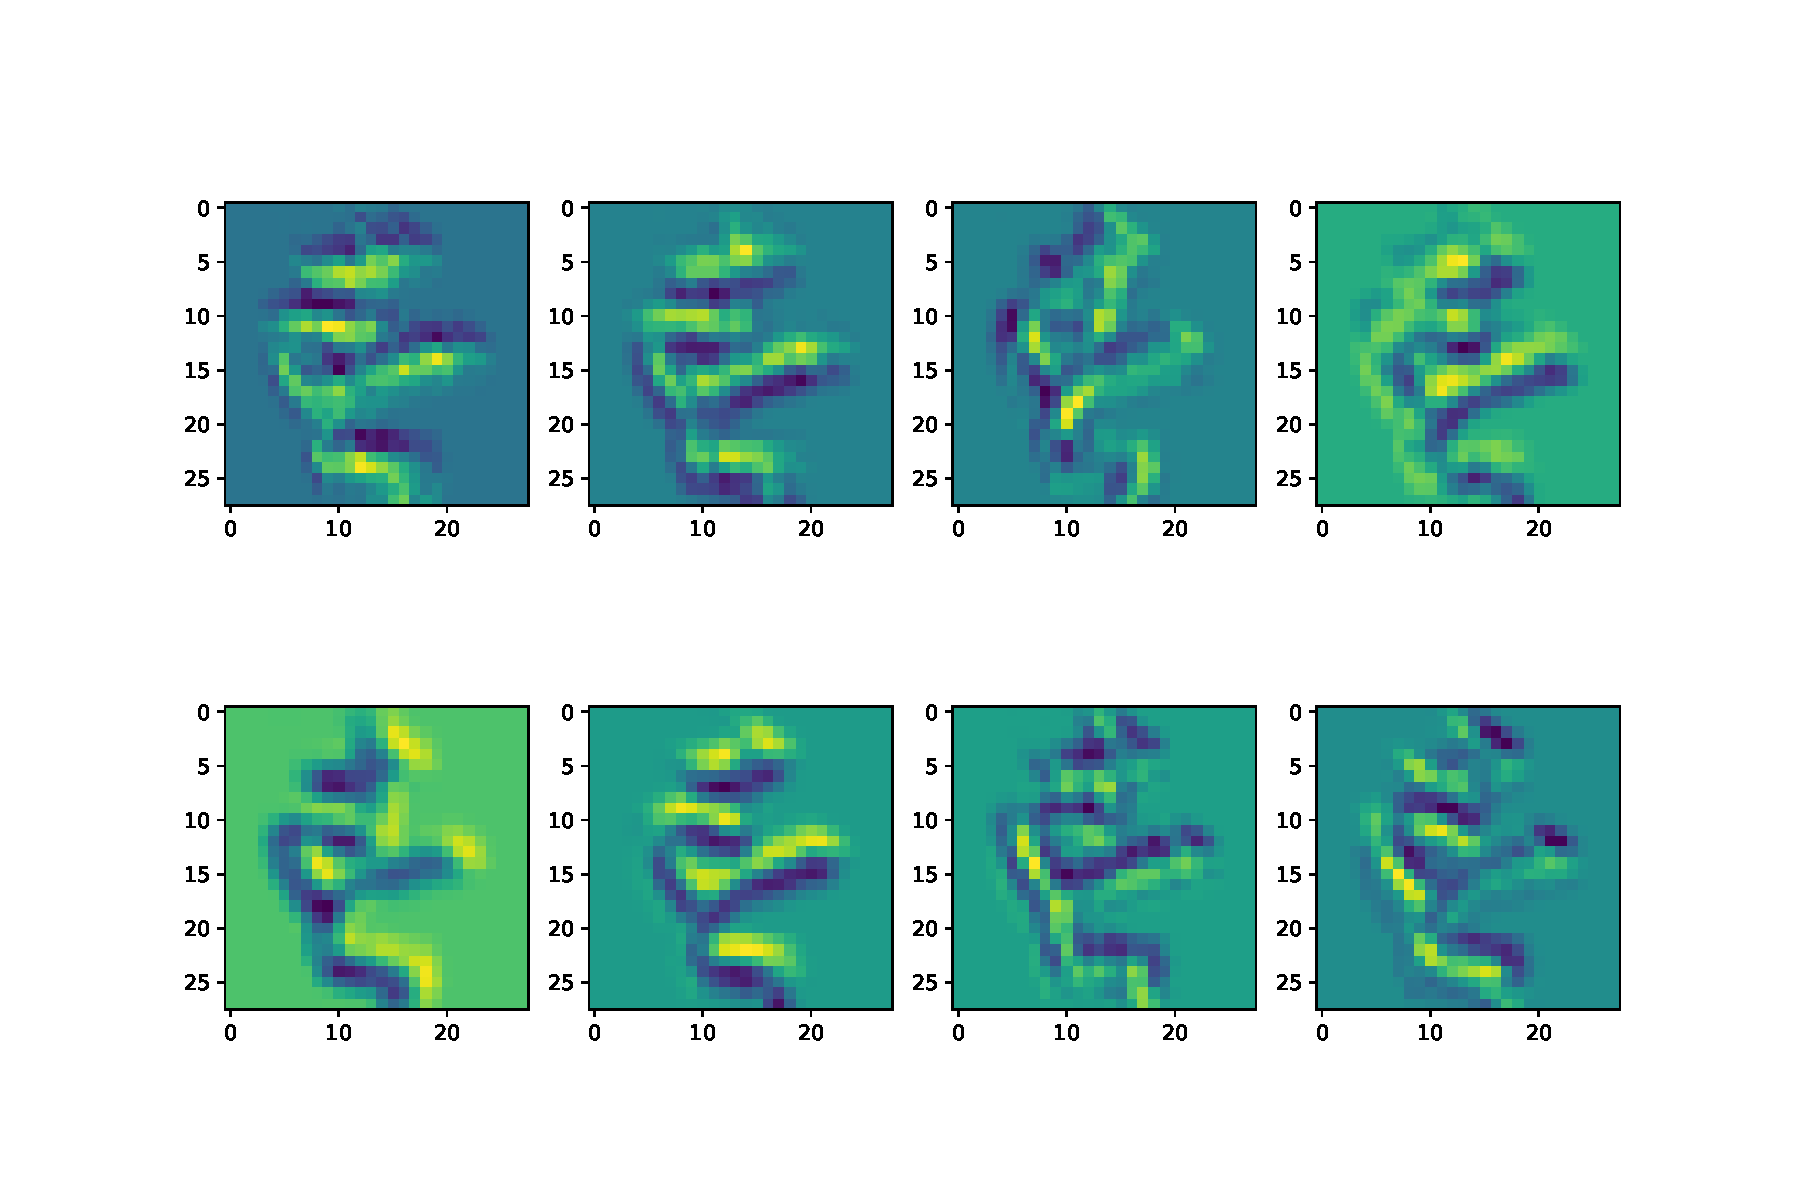
\includegraphics[width=1.5\linewidth]{activation_maps.pdf}
            %     \caption{Activation maps of the first convolutional layer}
            %     \label{fig:activation}
            %     \end{minipage}
            %     \hfill
            %     \begin{minipage}[c]{0.4\linewidth}
            %     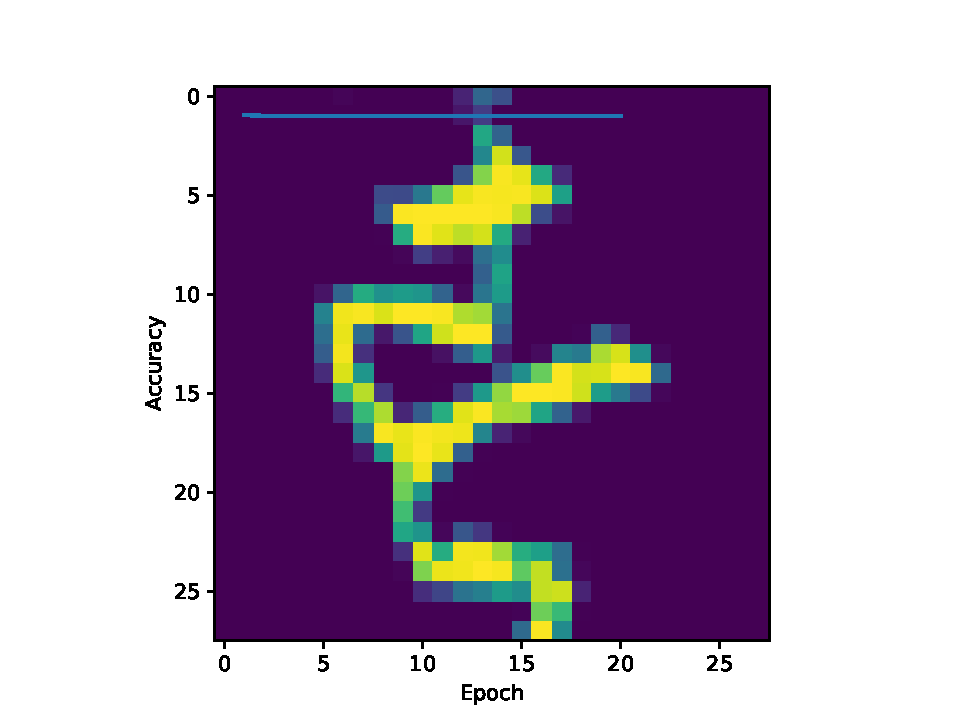
\includegraphics[width=1.2\linewidth]{original_image.pdf}
            %     \caption{Original Training Image}
                
            %     \label{fig:orig}
            %     \end{minipage}%
            % \end{figure}
            
            \begin{figure}[h]
                \centering
                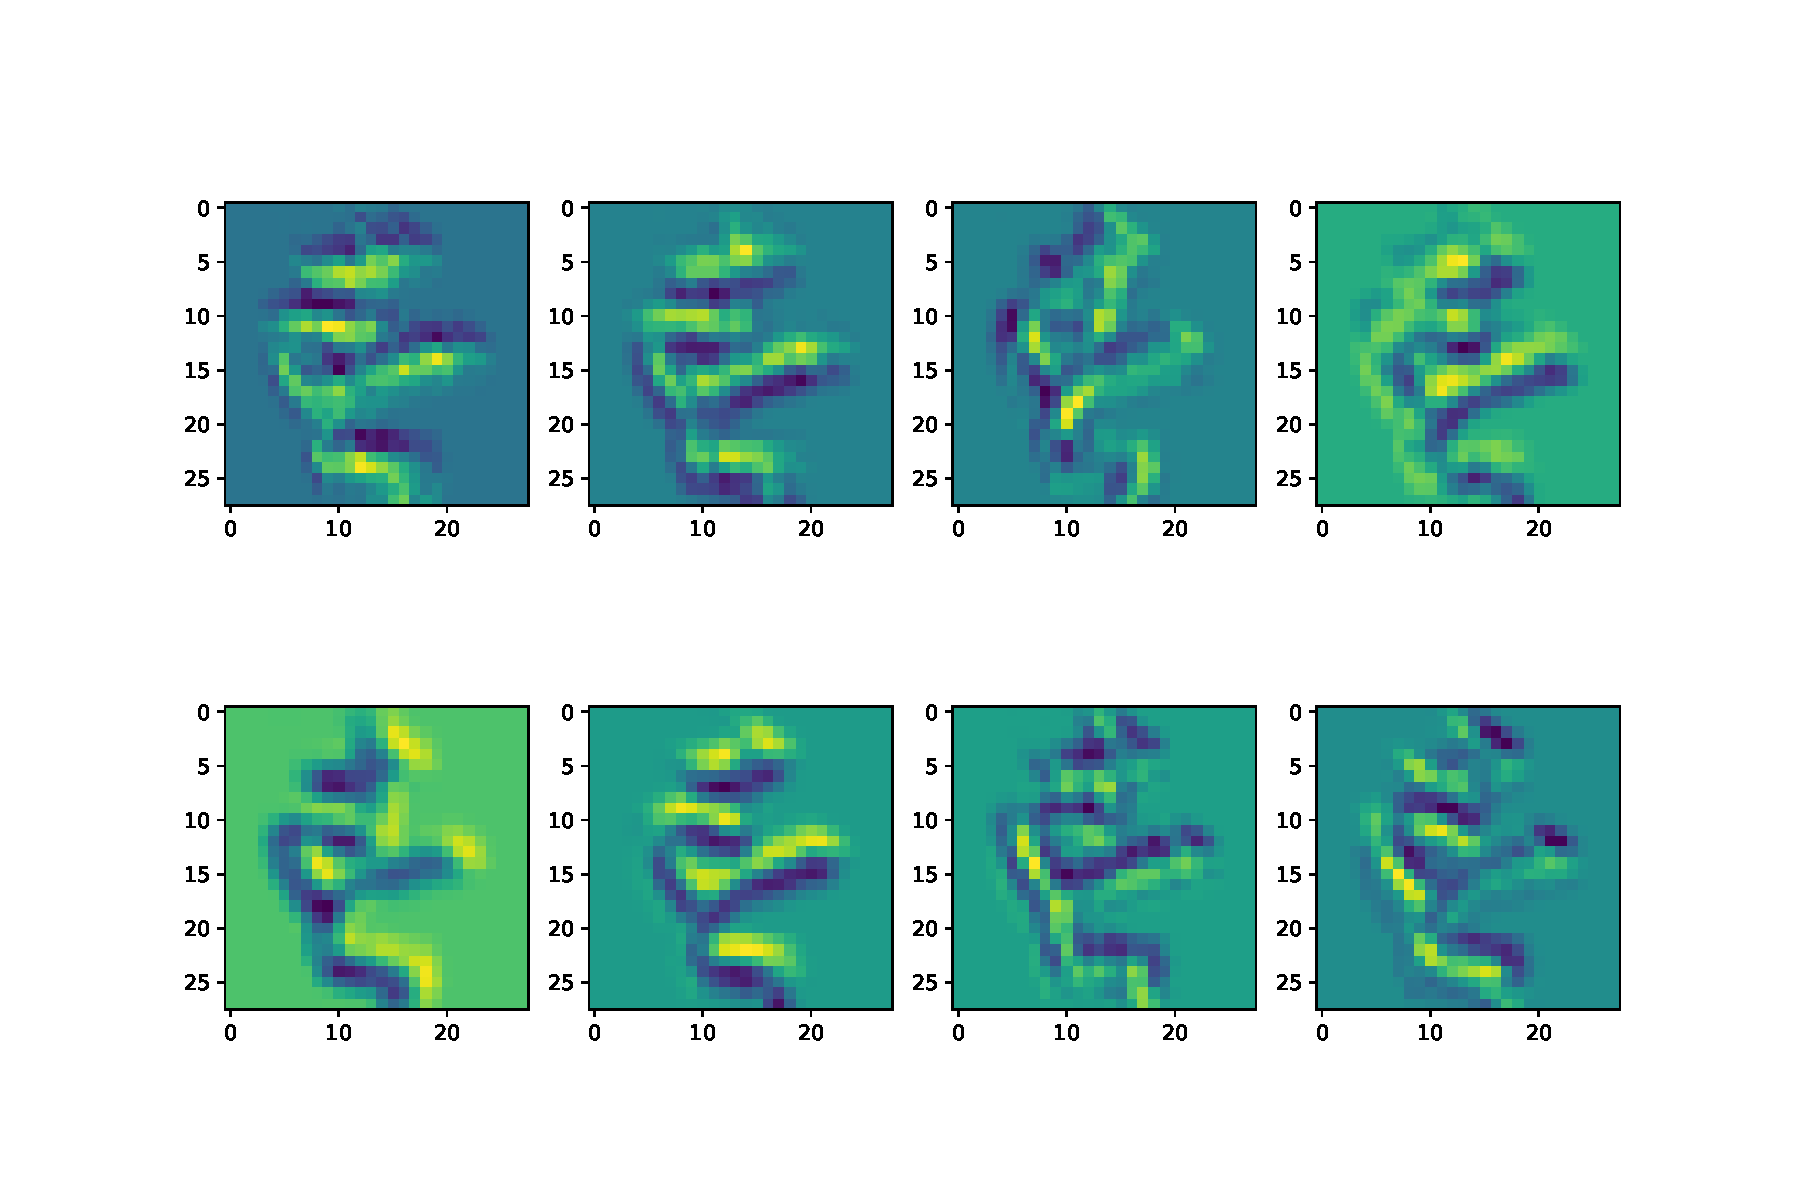
\includegraphics[scale=0.5]{activation_maps.pdf}
                \caption{Activation maps of the first convolutional layer}
                \label{fig:activation}
            \end{figure}
            \begin{figure}[h]
                \centering
                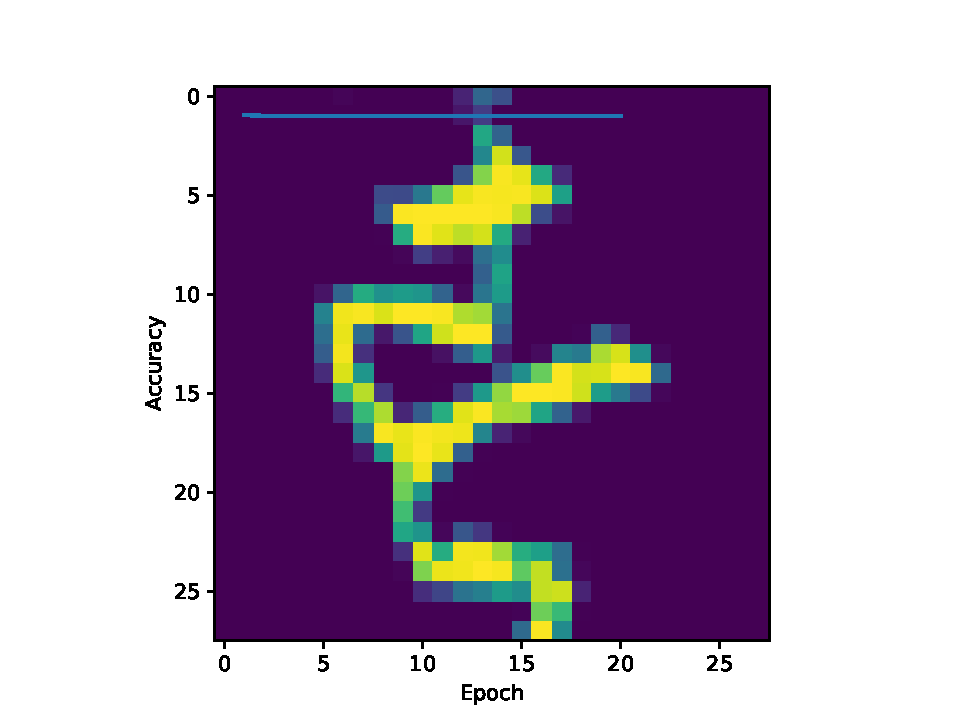
\includegraphics[scale=0.4]{original_image.pdf}
                \caption{Original Training Image}
                \label{fig:orig}
            \end{figure}
             Through the comparison of the various activation maps and the original training example, we can verify that each activation map highlights different sets of distinctive features of the character in the original image (namely, different sets of edges and corners appear yellow and dark blue in each activation map).


    \end{questions}

\clearpage
    \section*{Question 3}
    \begin{questions}
        \question
        \begin{parts}
            \part %3.1(a)
            After implementing the \texttt{forward()} methods for both the encoder and decoder, the model was trained over 50 epochs, using a learning rate of 0.003, a dropout rate of 0.3, a hidden size of 128, and a batch size of 64. The final validation error rate was 0.4995 and the final test error rate was 0.5001. The validation error rate over the epochs was also plotted.
            \begin{figure}[h]
                \centering
                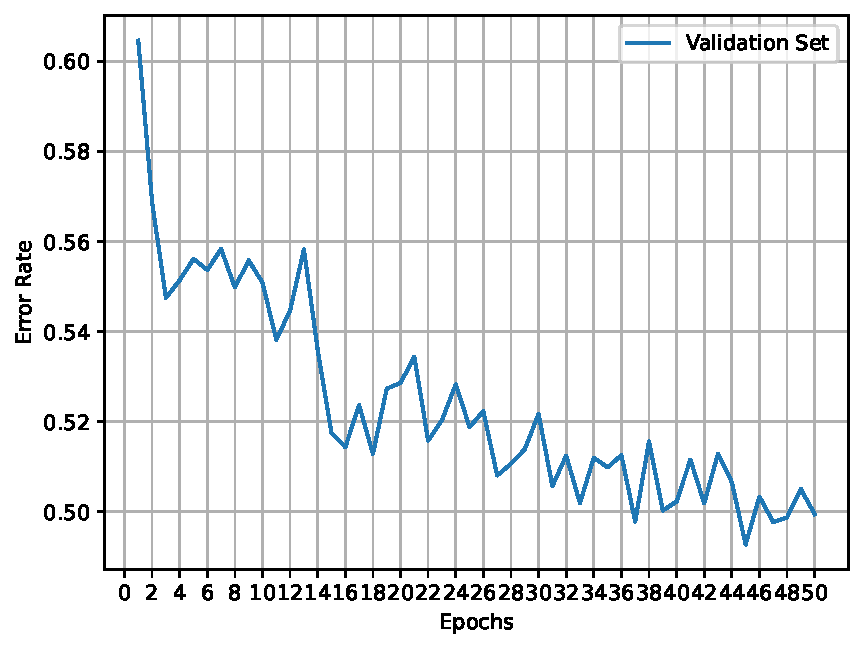
\includegraphics[scale=0.65]{pictures/attn_False_err_rate.pdf}
                \caption{Validation error rate over 50 epochs}
                \label{fig:3without_attn}
            \end{figure}

            \part %3.1(b)
            After adding the bilinear attention mechanism to the decoder, the model was trained with the same hyperparameters used in the previous exercise. The final validation error rate was 0.3523 and the final test error rate was 0.3629. The validation error rate over the epochs was also plotted.
            \begin{figure}[h]
                \centering
                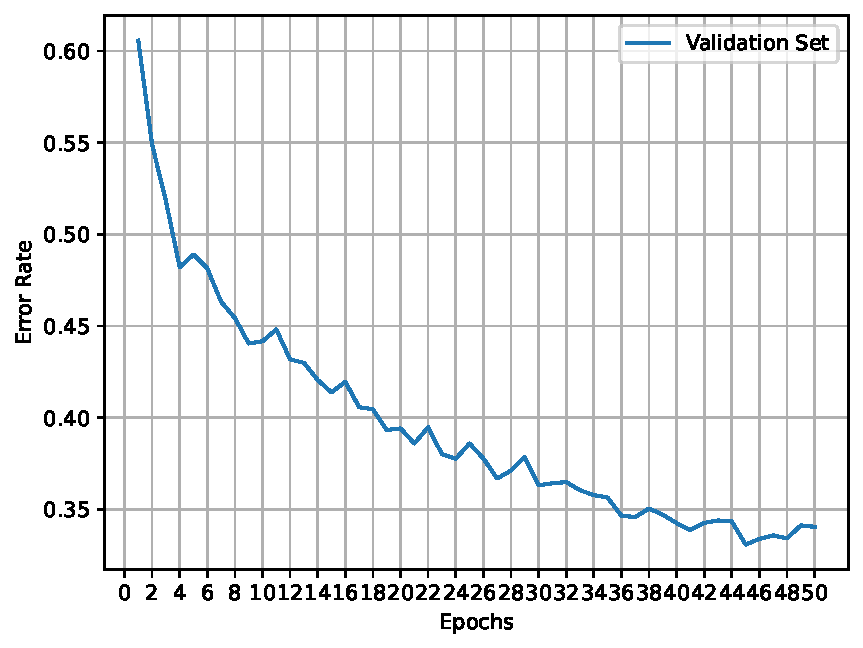
\includegraphics[scale=0.65]{pictures/attn_True_err_rate.pdf}
                \caption{Validation error rate over 50 epochs for the model with attention mechanism}
                \label{fig:3with_attn}
            \end{figure}
        \clearpage
            \part %3.1(c)
            At test time, given a source sequence $\vb*{x}$, the predicted target token is computed at time step $t$ in the following way:
            \[
            \hat{y}_t = \argmax_{y_t} \: \mathbb{P}(y_t | \text{START}, \hat{y}_1, \dots, \hat{y}_{t - 1}, \vb*{x})
            \]
            and thus a purely greedy search method is used to find $\argmax_{\vb*{y}} \: \mathbb{P}(\vb*{y} |\vb*{x})$ (i.e., the most probable target sequence given the source sequence). Not only does this approach greatly reduces the original search space, it can also critically compromise the rest of the predicted translated sequence once a wrong token is produced. Thus, we could obtain better translations while maintaining the used architecture simply by employing \textbf{beam search} with some beam size $k$, where $k$ is chosen so as to achieve a desirable balance between speed and accuracy. More specifically, at each time step $t$ we maintain a set of $k$ candidate partial target sequences $S_t = \{\vb*{y}_t^{(1)}, \dots, \vb*{y}_t^{(k)} \}$, with $S_0 = \{ \text{START} \}$. At each time step $t + 1$, we proceed to expand $S_t$ in the following way:
            \begin{align*}
                S^{*}_{t + 1} &= \bigcup_{i = 1}^{k} \left\{ (\vb*{y}_t^{(i)}, \hat{y}) \: | \: \hat{y} \in \argmax_{\hat{y}}^{k} \mathbb{P}(\hat{y} | \vb*{y}_t^{(i)}, \vb*{x})\right\} \\
                S_{t + 1} &= \argmax_{\vb*{y} \in S^{*}_{t + 1}}^{k} \mathbb{P}(\vb*{y} | \vb*{x})
            \end{align*}
            where the notation $\argmax_{x \in D}^k f(x)$ denotes the elements of $D$ that yield the $k$ largest values of $f(x)$ among all the elements of $D$. Thus, we can obtain better approximate solutions using this method, as it expands the search space in comparison to the previous method and mitigates the previous problem of sticking to a unique choice of $\hat{y}_t$ by maintaining various candidate partial target sequences.


        \end{parts}
    \end{questions}
\end{document}